\documentclass{article}
\usepackage[final,main,nonatbib]{neurips_2025}
\makeatletter
\renewcommand{\@noticestring}{}
\makeatother
\usepackage[utf8]{inputenc}
\usepackage[T1]{fontenc}
\usepackage{booktabs}
\usepackage{graphicx}
\graphicspath{{figures/}{../figures/}}
\usepackage{hyperref}
\usepackage{url}
\usepackage{microtype}
\usepackage{float}
\usepackage{caption}
\usepackage{longtable}
\title{Detecting Money Laundering with Transaction and Account Graph Features}
\author{Bokang GAO \quad Zi Xuan SZETO \quad Minghua XIONG \\
Group: zxszeto's group (zxszeto\_group)}
\date{}
\begin{document}
\maketitle

\section{Introduction}
This project studies the IBM synthetic AML transaction dataset. The full dataset contains 5,078,345 transactions, 5,177 laundering labels, and a positive rate of 0.1019\%. The central question is whether account graph features help after accounting for class imbalance and leakage risk.

\begin{table}[H]
\centering
\caption{Failure-driven experiment path.}
\resizebox{\textwidth}{!}{%
\begin{tabular}{llll}
\toprule
Attempt & Observed failure & Next decision & Result \\
\midrule
All-legitimate & High accuracy, zero recall & Use rare-event metrics & F1 and PR-AUC emphasized \\
LR / Linear SVM & Weak PR-AUC & Try nonlinear models & Tree/RF/HGB \\
Decision Tree & Many false positives & Use ensembles & More stable ranking \\
Base RF/HGB & No account context & Add graph features & Random-split PR-AUC improves \\
Natural prior & Precision collapses & Alert-budget sweep & Operational trade-off exposed \\
Time split & Graph lift reverses & Audit leakage risk & Bounded deployment claim \\
\bottomrule
\end{tabular}
}
\end{table}

\section{Dataset and Experimental Protocol}
The official dataset source is Kaggle/IBM. The scripts use a Hugging Face mirror only as a programmatic fallback. Full-data chunked statistics are used for EDA. t-SNE and DBSCAN are sampled for computational feasibility. Supervised modeling uses a stratified modeling sample containing all laundering transactions and sampled legitimate transactions.

Three evaluations answer different questions. (1) The \emph{random/transductive sampled evaluation} compares models and ablations on the modeling sample. (2) The \emph{natural class-prior stress test} restores the full-data base rate to expose alert pressure. (3) The \emph{time-based leakage audit} orders the modeling sample by time and constructs graph statistics from training history only. These are separate protocols, not three views of one test set.

\section{Mandatory Tasks}
\subsection{Preprocessing and EDA}
We check missing values and duplicates, parse timestamps, one-hot encode currency and payment format, and standardize numeric features. Engineered transaction-level features include amount, log amount, hour, weekday, same-bank flag, and same-currency flag.

\subsection{t-SNE Visualization}
\begin{figure}[H]
\centering
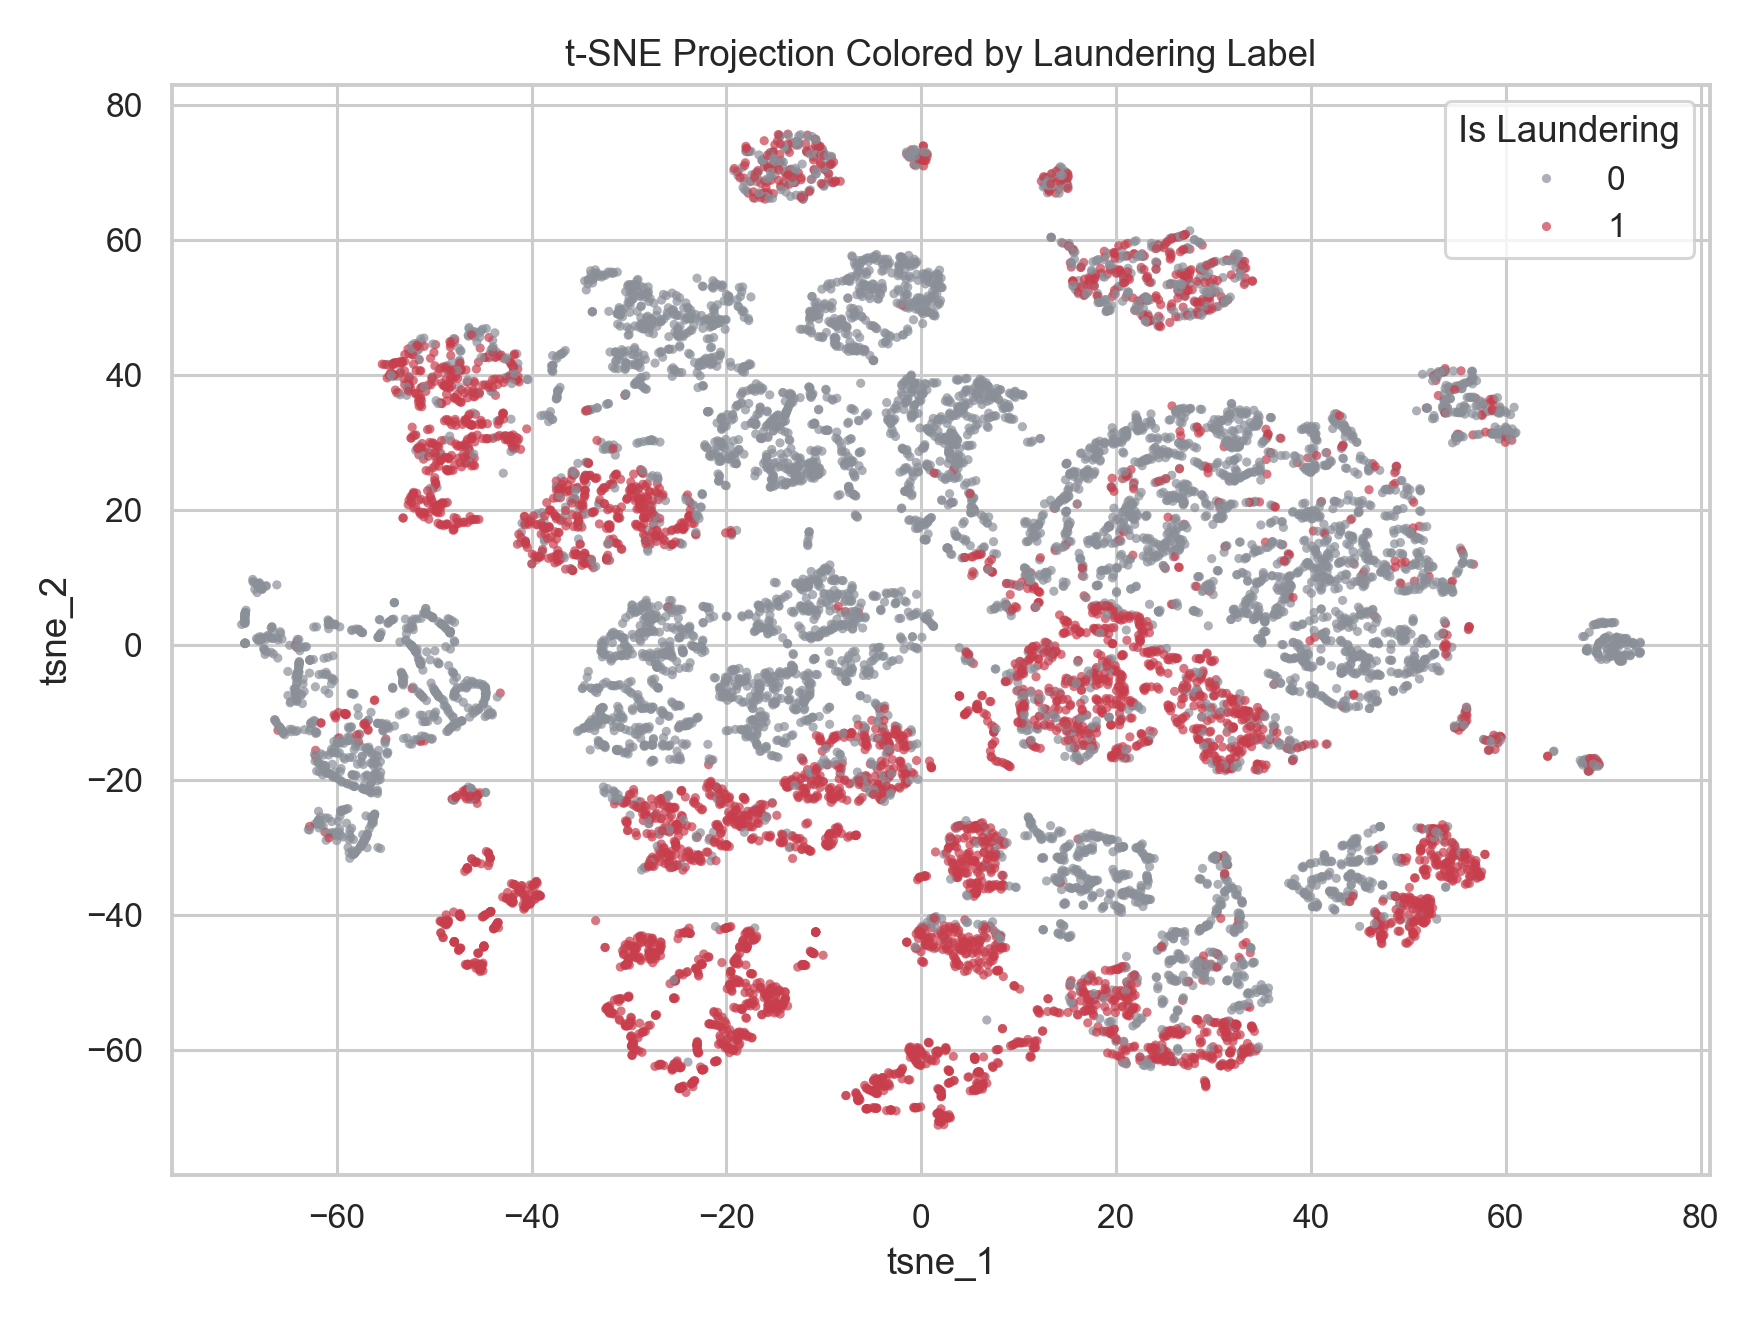
\includegraphics[width=0.82\linewidth]{tsne_projection.png}
\caption{t-SNE projection on a stratified transaction sample. Laundering samples form local neighborhoods but still overlap with legitimate transactions, so visualization does not replace supervised learning.}
\end{figure}

\subsection{KMeans and DBSCAN Clustering}
KMeans and DBSCAN are applied to account-level behavior features. Purity is inflated by class imbalance, so it must be interpreted together with NMI and ARI.
\begin{figure}[H]
\centering
\begin{minipage}[t]{0.49\linewidth}
\centering
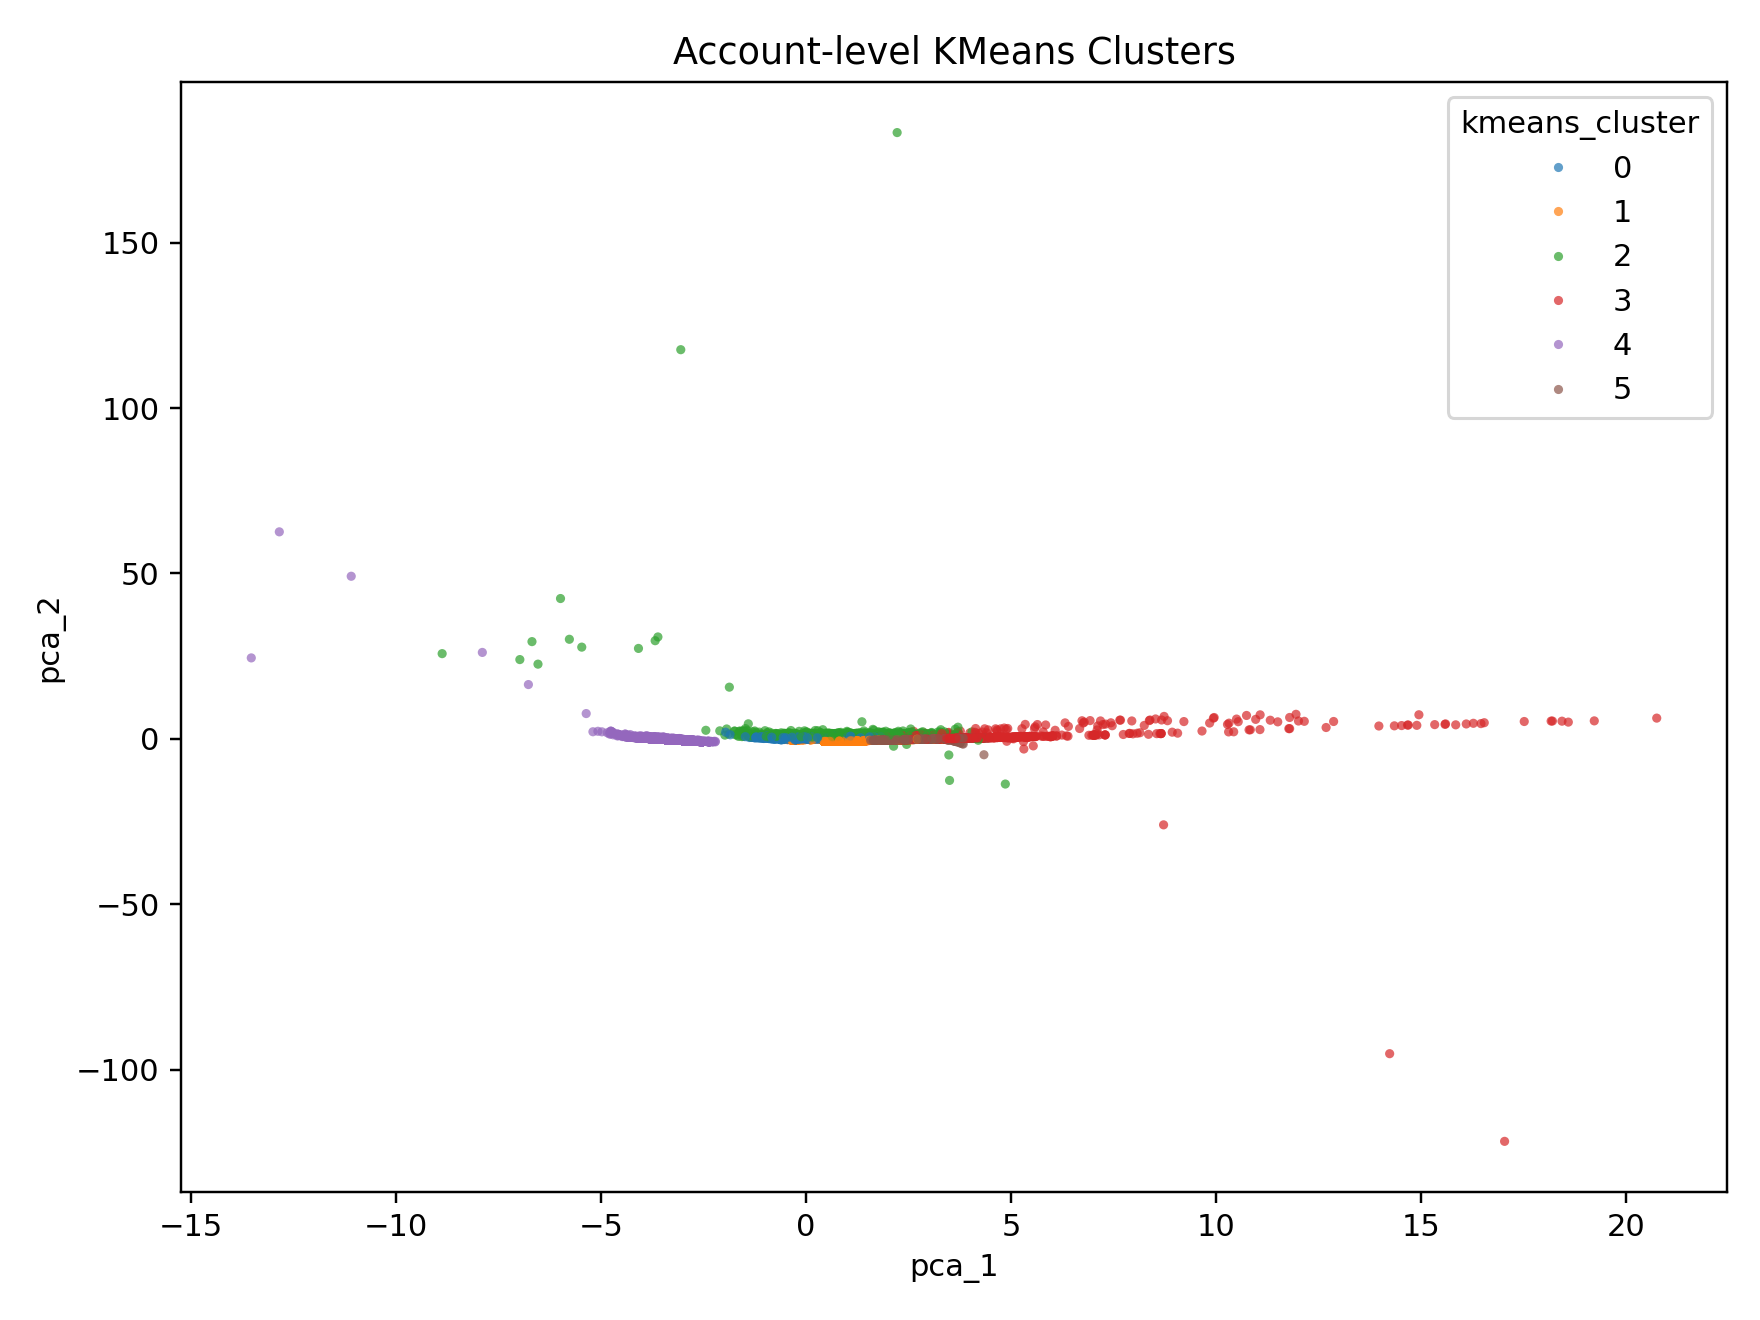
\includegraphics[width=\linewidth]{account_kmeans_clusters.png}\\[-2mm]
\footnotesize (a) Account-level KMeans clusters
\end{minipage}
\hfill
\begin{minipage}[t]{0.49\linewidth}
\centering
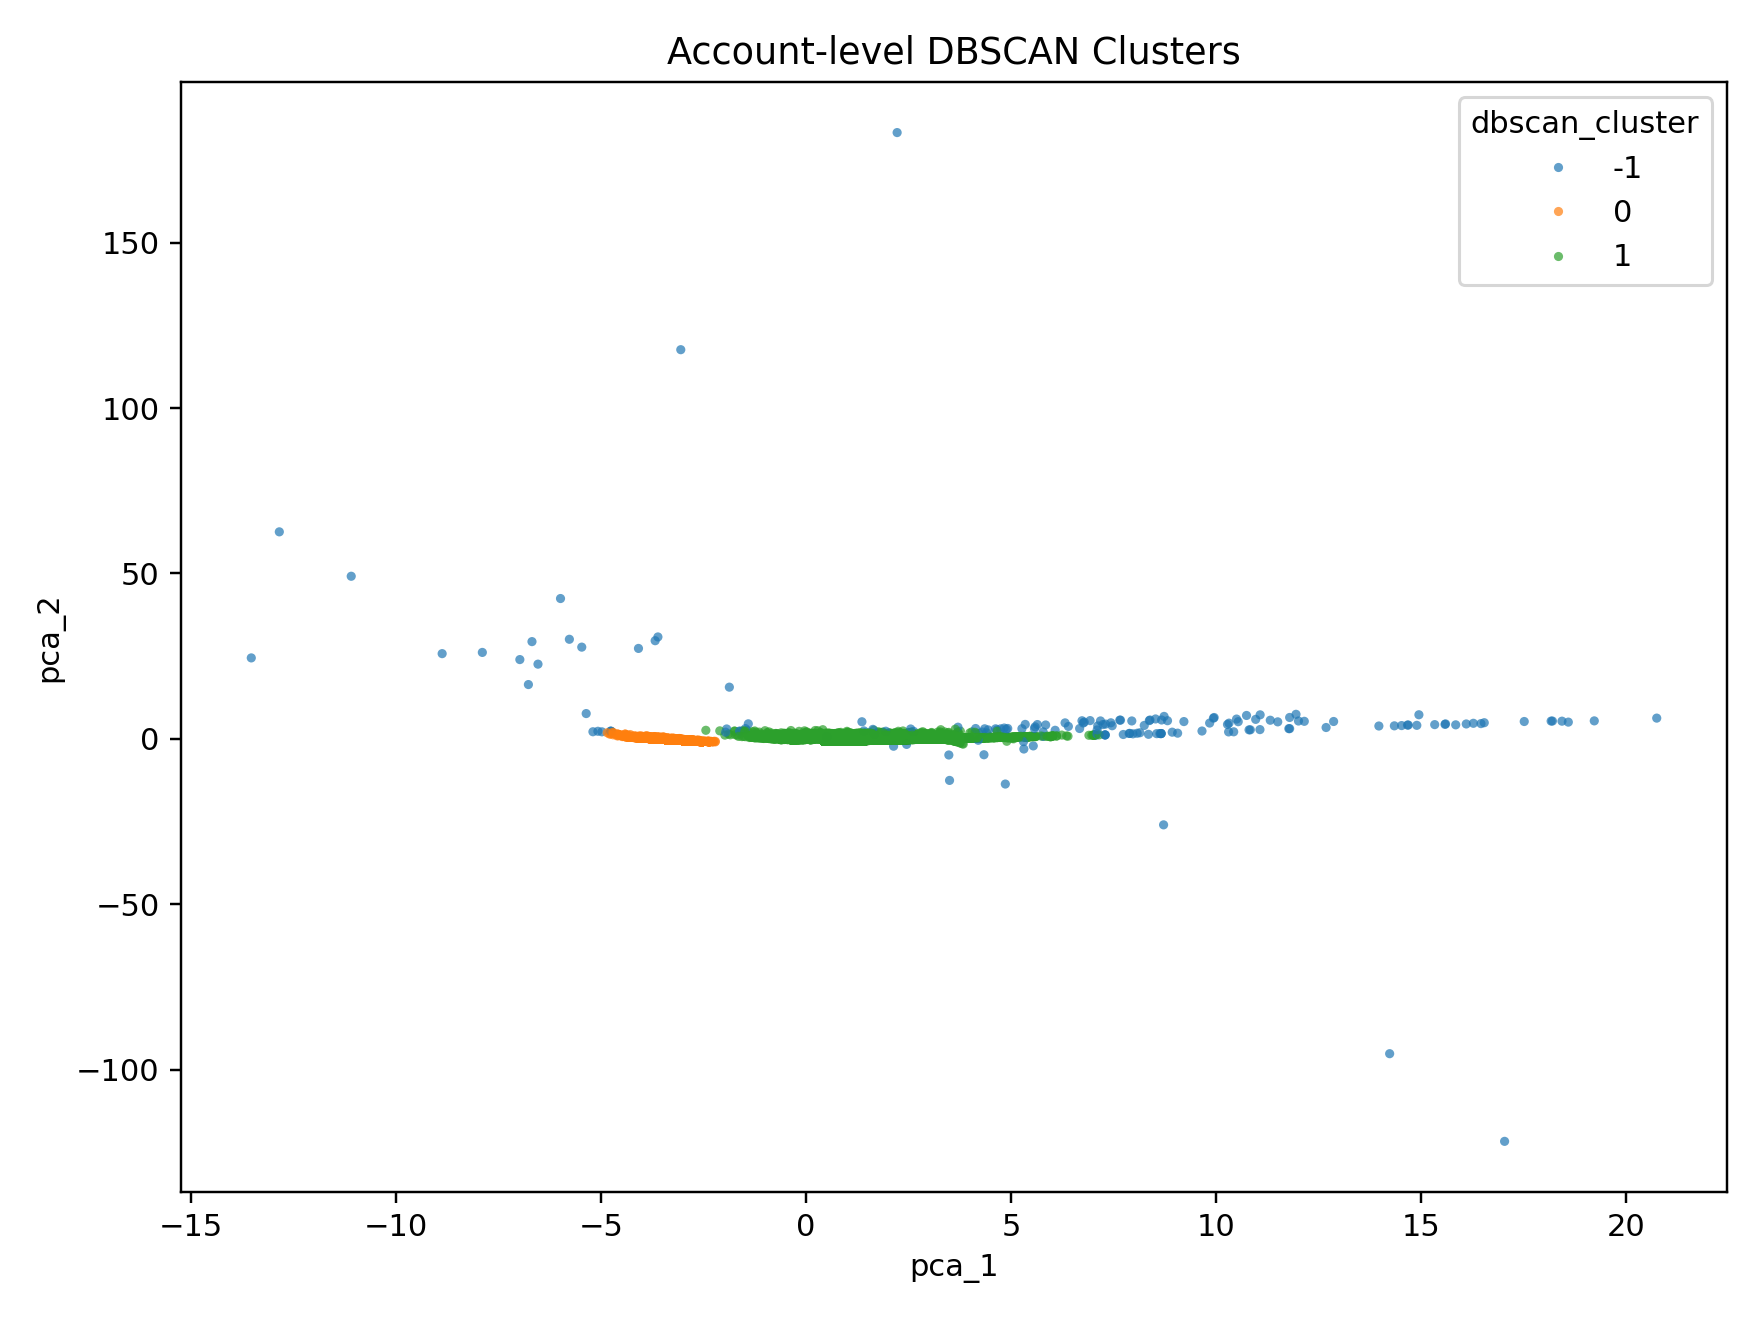
\includegraphics[width=\linewidth]{account_dbscan_clusters.png}\\[-2mm]
\footnotesize (b) Account-level DBSCAN clusters
\end{minipage}
\caption{Cluster-label visualizations using account-level behavior features. DBSCAN isolates a small high-risk noise/outlier group (label $-1$) in the modeling account sample, but both methods have very low NMI/ARI and therefore cannot replace supervised labels. Purity is also inflated by class imbalance.}
\end{figure}

\begin{table}[H]
\centering
\caption{Account-level clustering metrics.}
\resizebox{\textwidth}{!}{%
\begin{tabular}{lrrrrr}
\toprule
Method & Sil. & NMI & ARI & Purity & Max risk \\
\midrule
Account KMeans & 0.380 & 0.021 & 0.017 & 0.759 & 0.424 \\
Account DBSCAN & 0.478 & 0.001 & -0.008 & 0.763 & 0.848 \\
\bottomrule
\end{tabular}
}
\end{table}

\subsection{Supervised Model Training and Validation}
We compare Dummy All-Legitimate, Logistic Regression, Linear SVM, Decision Tree, Random Forest, and HistGradientBoosting. Thresholds are selected on a validation split inside the training set.
\begin{table}[H]
\centering
\caption{Sampled-test model comparison.}
\resizebox{\textwidth}{!}{%
\begin{tabular}{lrrr}
\toprule
Model & F1 & ROC-AUC & PR-AUC \\
\midrule
HistGradientBoosting + Graph Features & 0.628 & 0.976 & 0.721 \\
Random Forest + Graph Features & 0.591 & 0.972 & 0.681 \\
HistGradientBoosting Base Features & 0.540 & 0.930 & 0.556 \\
Random Forest Base Features & 0.529 & 0.927 & 0.550 \\
Decision Tree & 0.469 & 0.906 & 0.405 \\
Linear SVM & 0.459 & 0.915 & 0.327 \\
Logistic Regression & 0.459 & 0.915 & 0.338 \\
Dummy All-Legitimate & 0.000 & 0.500 & 0.031 \\
\bottomrule
\end{tabular}
}
\end{table}

\begin{figure}[H]
\centering
\begin{minipage}[t]{0.49\linewidth}
\centering
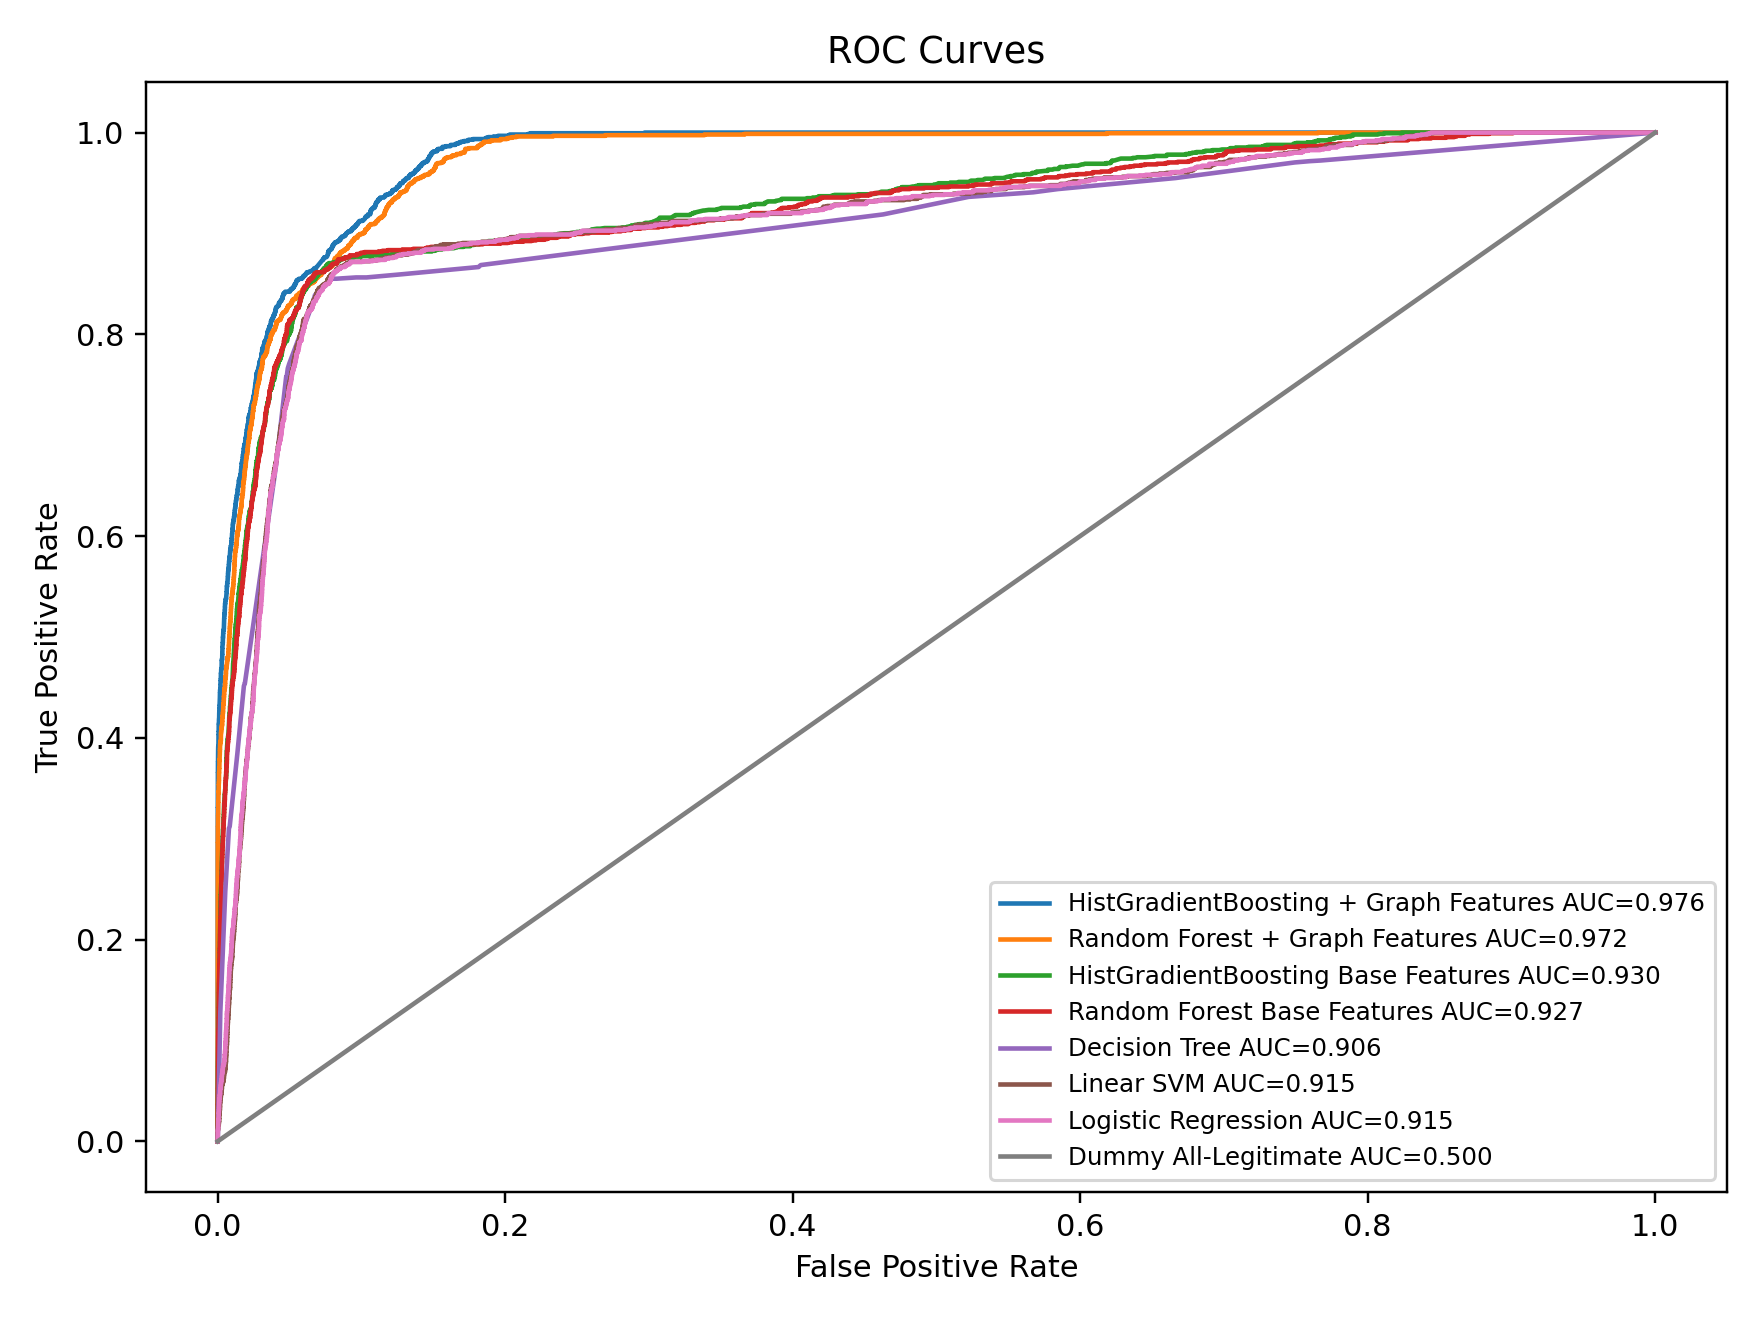
\includegraphics[width=\linewidth]{roc_curves.png}\\[-2mm]
\footnotesize (a) ROC curves
\end{minipage}
\hfill
\begin{minipage}[t]{0.49\linewidth}
\centering
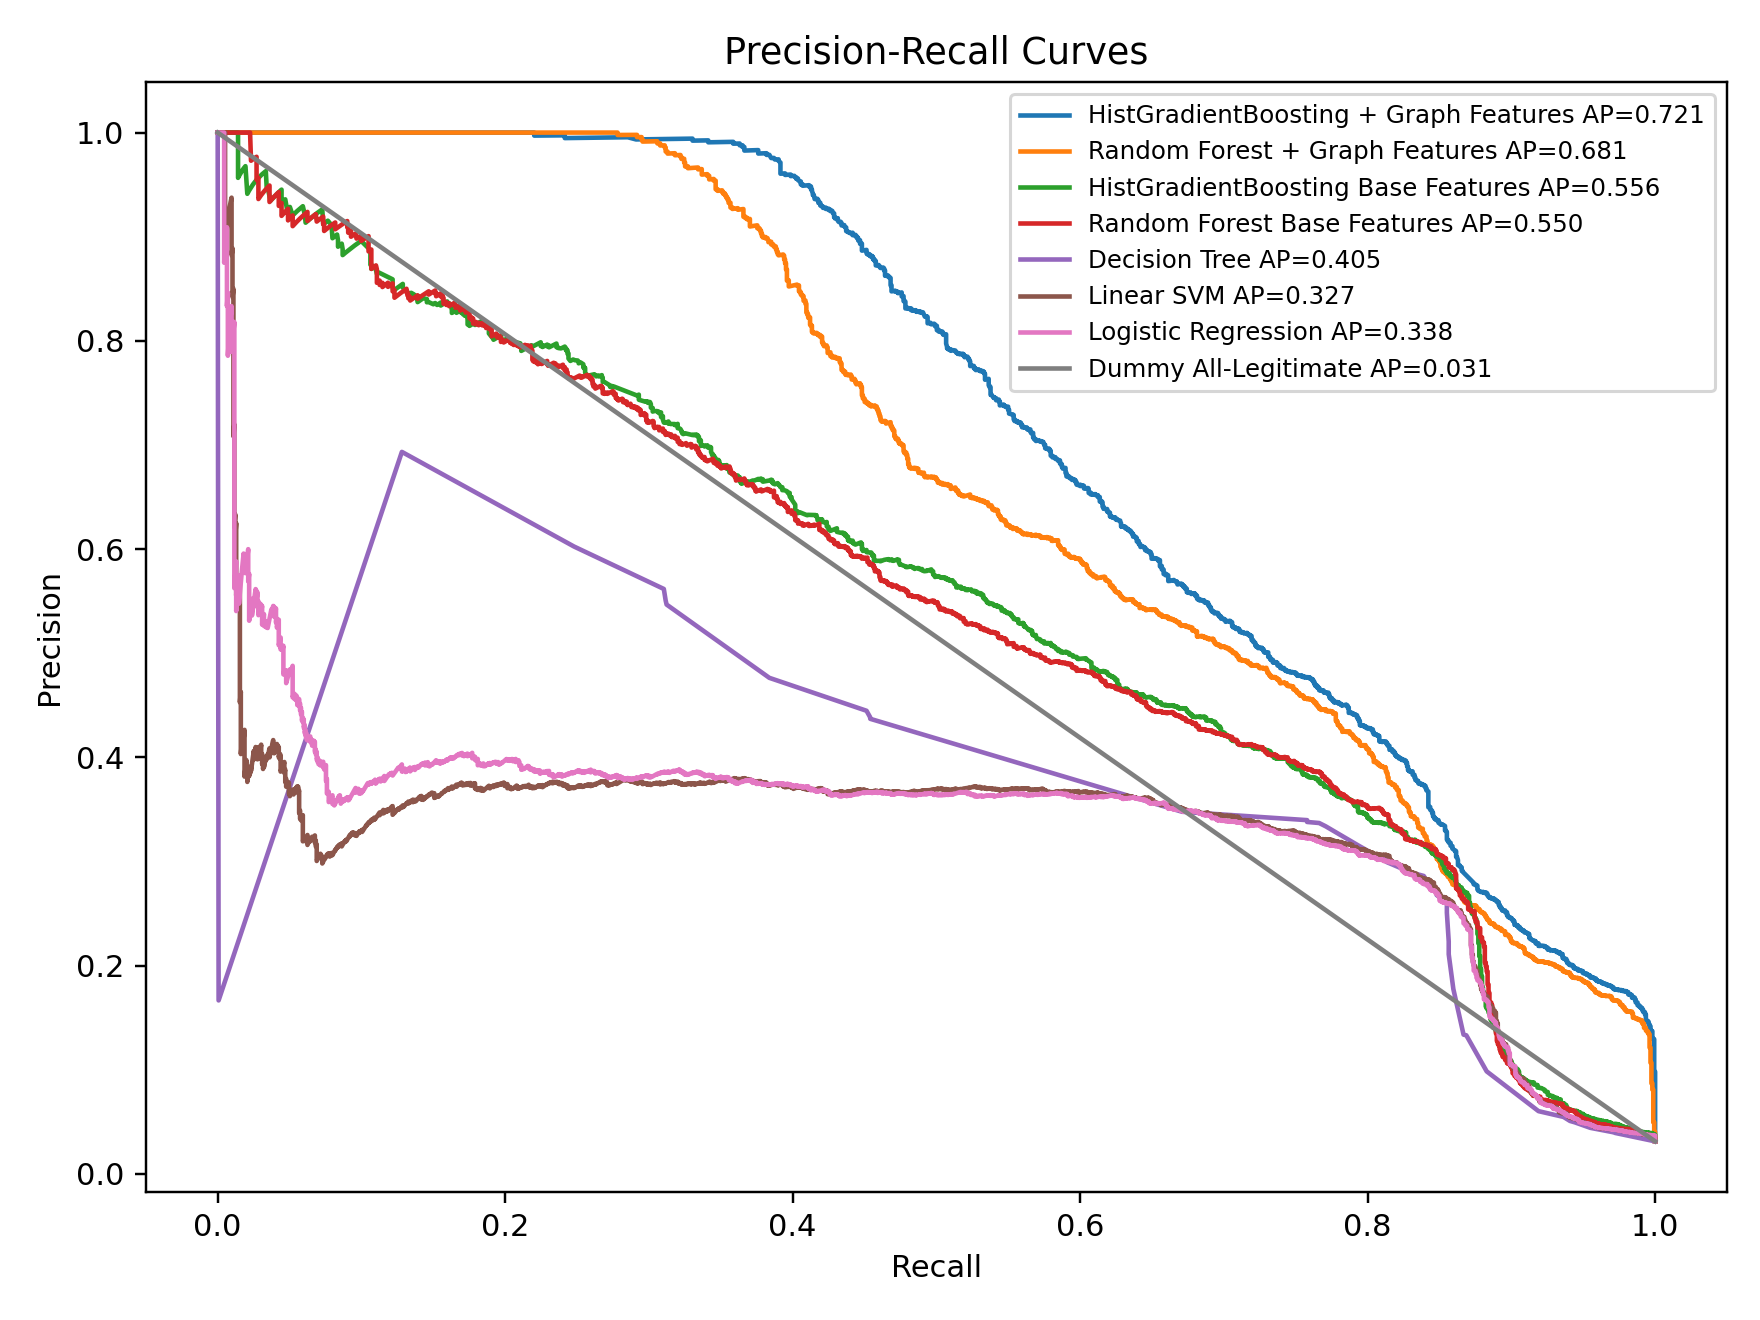
\includegraphics[width=\linewidth]{pr_curves.png}\\[-2mm]
\footnotesize (b) Precision--recall curves
\end{minipage}
\caption{Sampled-test ROC and precision--recall curves. ROC-AUC provides the standard ranking evaluation required by the course, while PR-AUC is more informative under severe AML imbalance. Accuracy alone is misleading because an all-legitimate classifier is highly accurate on the full data but has zero recall and zero F1.}
\end{figure}

\begin{table}[H]
\centering
\caption{Train, test, and full modeling-sample evaluation for the selected HistGradientBoosting + Graph Features model.}
\resizebox{\textwidth}{!}{%
\begin{tabular}{lrrrrr}
\toprule
Split & Precision & Recall & F1 & ROC-AUC & PR-AUC \\
\midrule
Train & 0.712 & 0.634 & 0.671 & 0.984 & 0.771 \\
Test & 0.670 & 0.590 & 0.628 & 0.976 & 0.721 \\
Full modeling sample & 0.699 & 0.621 & 0.658 & 0.982 & 0.756 \\
\bottomrule
\end{tabular}
}
\end{table}

\begin{figure}[H]
\centering
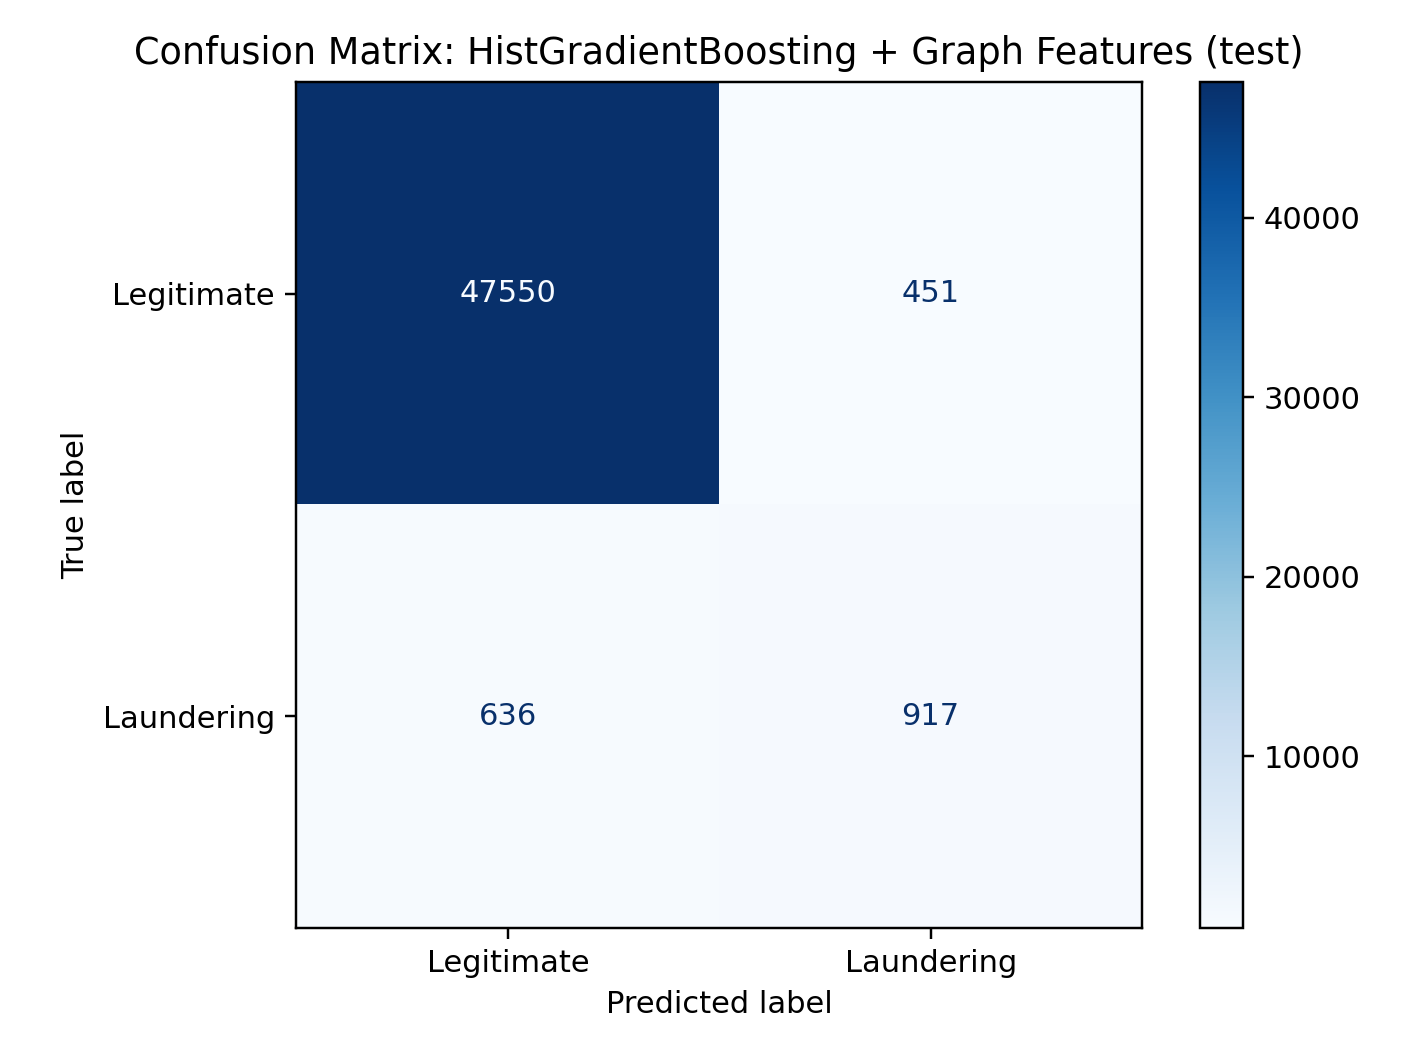
\includegraphics[width=0.62\linewidth]{confusion_matrix_histgradientboosting_plus_graph_features_test.png}
\caption{Sampled-test confusion matrix for the HistGradientBoosting model with graph features. This matrix makes the trade-off between recovered laundering transactions and false alerts explicit.}
\end{figure}
Train and full-sample confusion matrices are provided in the executed notebook.

\section{Open-ended Exploration}
\subsection{Account Graph Feature Engineering}
Account features include in/out degree, unique counterparties, total sent/received amount, PageRank, fan-in, fan-out, and scatter-gather proxies.

\subsection{Model and Feature Ablation}
The main random/transductive split result is HGB + Graph with F1=0.628, ROC-AUC=0.976, and PR-AUC=0.721. Adding graph features changes Random Forest F1 by +0.062 and PR-AUC by +0.131; for HGB the changes are +0.088 F1 and +0.166 PR-AUC. These random/transductive gains should not be overstated as deployment improvement.

\subsection{Mutual-information Top-k Feature Selection}
\begin{table}[H]
\centering
\caption{Top-k mutual-information feature selection with retraining.}
\resizebox{\textwidth}{!}{%
\begin{tabular}{lrrrr}
\toprule
Feature set & N & F1 & PR-AUC & Train sec \\
\midrule
All base+graph encoded features & 60 & 0.628 & 0.721 & 2.41 \\
Top-5 mutual information features & 5 & 0.515 & 0.569 & 0.89 \\
Top-10 mutual information features & 10 & 0.564 & 0.656 & 0.91 \\
Top-20 mutual information features & 20 & 0.604 & 0.699 & 1.16 \\
All base features (pipeline result) &  & 0.540 & 0.556 &  \\
All graph features (pipeline result) &  & 0.628 & 0.721 &  \\
\bottomrule
\end{tabular}
}
\end{table}
Top-20 MI features retain most sampled-test performance while reducing feature dimensionality and training time.

\subsection{Natural Class-prior Stress Test}
The natural class-prior stress test contains 1,501,553 rows, positive rate 0.1034\%, precision 0.83\%, recall 53.70\%, F1 0.016, ROC-AUC 0.907, PR-AUC 0.009, FP 99,113, and TP 834. It triggers 665.6 alerts per 10,000 transactions. This experiment primarily isolates the effect of restoring the natural class prior. It is not a fully independent temporal deployment evaluation because evaluation sampling and graph-statistic construction may retain transductive elements.

\begin{figure}[H]
\centering
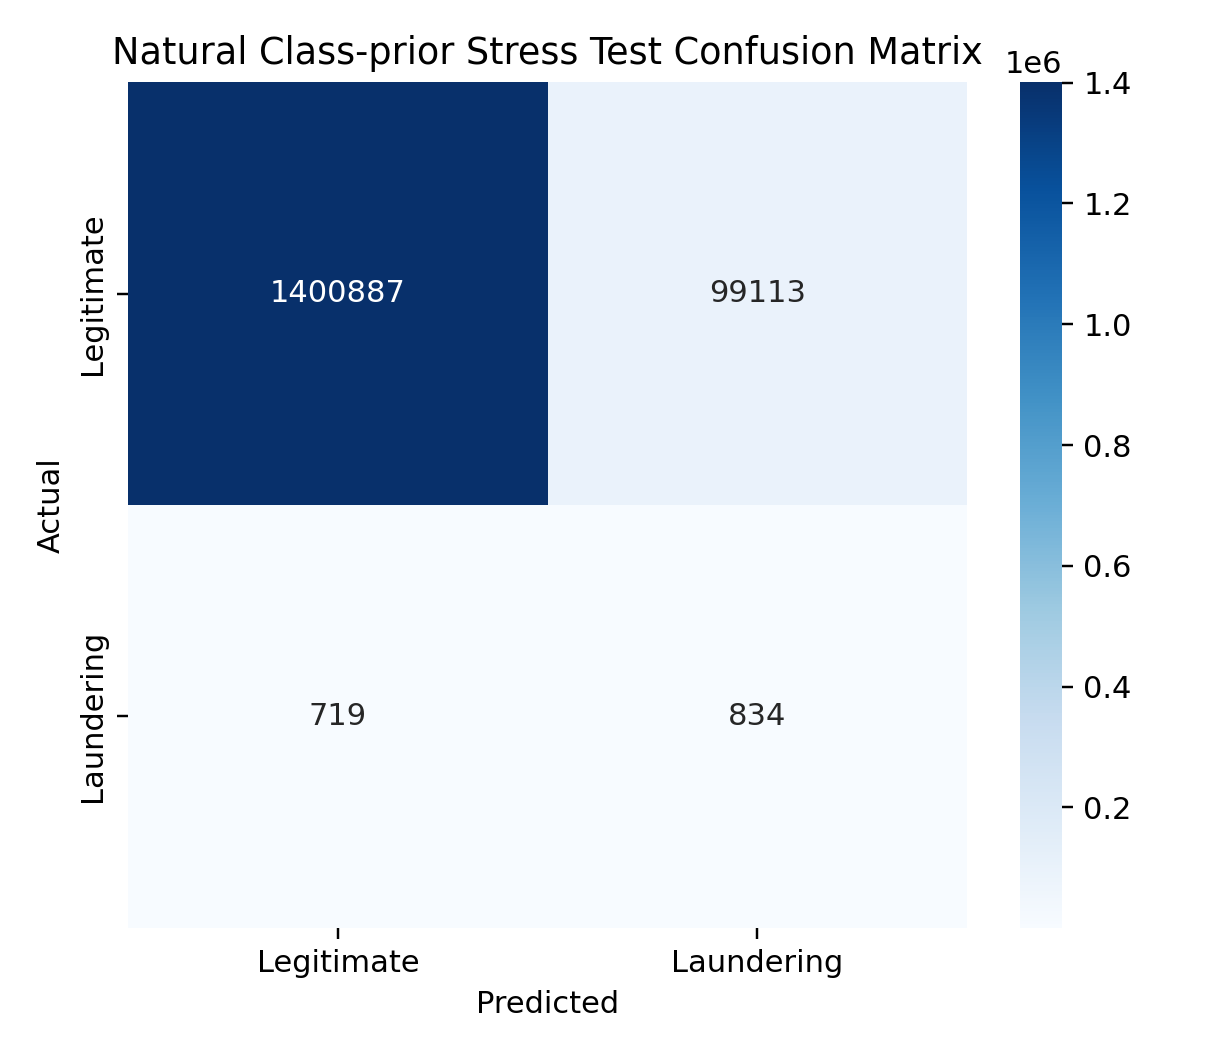
\includegraphics[width=0.88\linewidth]{confusion_matrix_natural_distribution.png}
\caption{Natural class-prior stress-test confusion matrix. Even a strong sampled-test model produces many false positives when evaluated against the full-data base rate, which motivates alert-budget threshold analysis.}
\end{figure}

\subsection{Time-based Leakage Audit}
\begin{table}[H]
\centering
\caption{Random/transductive graph gains are audited with a time-based split.}
\resizebox{\textwidth}{!}{%
\begin{tabular}{llrr}
\toprule
Protocol & Model & F1 & PR-AUC \\
\midrule
time\_based\_60\_20\_20 & HGB Base, time split & 0.662 & 0.683 \\
time\_based\_60\_20\_20 & HGB Graph, time split with train-only graph features & 0.483 & 0.459 \\
\bottomrule
\end{tabular}
}
\end{table}
The time split is conducted on the modeling sample, whose positive rate is approximately 5.32\%; it is a leakage audit rather than a natural-prior deployment simulation. HGB Base obtains F1=0.662 and PR-AUC=0.683, whereas HGB Graph falls to F1=0.483 and PR-AUC=0.459. Graph behavior features are promising, but random-split gains are sensitive to protocol design. Rolling historical graph features are needed before making deployment claims.

\section{Discussion and Limitations}
Limitations include the synthetic AML dataset, strong class imbalance, random-split transductive leakage risk, natural-prior stress test not being a fully independent temporal test, time-split modeling sample positive rate of 5.32\%, operational alert-budget calibration, and lack of rolling historical graph construction.

\section{Conclusion}
The project completes preprocessing, t-SNE, KMeans/DBSCAN clustering, supervised model training, validation, train/test/full evaluation, ROC/AUC, graph-feature ablation, top-k feature selection, natural class-prior stress testing, and leakage auditing. The final claim is bounded: graph features help in random/transductive sampled evaluation, but deployment claims require stricter temporal protocols.

\section{References}
\begin{enumerate}
\item IBM AML-Data GitHub repository. \url{https://github.com/IBM/AML-Data}
\item Kaggle IBM Transactions for Anti Money Laundering dataset. \url{https://www.kaggle.com/datasets/ealtman2019/ibm-transactions-for-anti-money-laundering-aml}
\item E. Altman, J. Blanu\v{s}a, L. von Niederh\"ausern, B. Egressy, A. Anghel, and K. Atasu. Realistic Synthetic Financial Transactions for Anti-Money Laundering Models. NeurIPS Datasets and Benchmarks, 2023.
\item B. Deprez, T. Vanderschueren, B. Baesens, T. Verdonck, and W. Verbeke. Network Analytics for Anti-money Laundering---A Systematic Literature Review and Experimental Evaluation. INFORMS Journal on Data Science, published online 2025.
\item J. Blanu\v{s}a, M. Cravero Baraja, A. Anghel, L. von Niederh\"ausern, E. Altman, H. Pozidis, and K. Atasu. Graph Feature Preprocessor: Real-time Subgraph-based Feature Extraction for Financial Crime Detection. ACM ICAIF, 2024.
\item M. Di Gennaro, F. Panebianco, M. Pianta, S. Zanero, and M. Carminati. Amatriciana: Exploiting Temporal GNNs for Robust and Efficient Money Laundering Detection. IEEE ICDM Workshops, 2024.
\end{enumerate}

\section{Credit and GenAI Disclosure}
Team contributions: Minghua XIONG was responsible for data processing. Bokang GAO and Zi Xuan SZETO were responsible for the remaining project components, including exploratory analysis, feature engineering, clustering, supervised modeling, model and feature ablation, natural class-prior stress testing, leakage auditing, report preparation, presentation design, and notebook integration.

GenAI disclosure: Codex/ChatGPT was used for planning, debugging, visualization/report structuring, and language polishing. The team verified the code outputs, numerical results, and final interpretation. Estimated GenAI-assisted content: 25\%.

\end{document}
